\documentclass[preprint,12pt]{elsarticle}

\journal{International Journal of Intelligent Networks}

% -------------------- Packages --------------------
\usepackage{cite}
\usepackage{amsmath,amssymb,amsfonts,amsthm,mathtools,bm}
\usepackage{algorithm}
\usepackage{algpseudocode}
\usepackage{graphicx}
\usepackage{textcomp}
\usepackage{xcolor}
\usepackage{booktabs}
\usepackage{multirow}
\usepackage{url}
\usepackage{array}
\usepackage{enumitem}
\usepackage{makecell}
\usepackage{tabularx}
\usepackage{siunitx}
\usepackage{microtype}
\usepackage[hidelinks]{hyperref}
\usepackage{tikz}
\usetikzlibrary{shapes.geometric,arrows.meta,positioning,backgrounds,calc,fit,matrix}
\usepackage{pgfplots}
\pgfplotsset{compat=1.17}

% -------------------- Theorem Environments --------------------
\newtheorem{theorem}{Theorem}
\newtheorem{proposition}{Proposition}
\newtheorem{remark}{Remark}
\newtheorem{assumption}{Assumption}
\newtheorem{lemma}{Lemma}

\DeclareMathOperator*{\argmin}{arg\,min}
\DeclareMathOperator*{\argmax}{arg\,max}
\DeclareMathOperator{\E}{\mathbb{E}}
\DeclareMathOperator{\KL}{D_{\mathrm{KL}}}

\sisetup{detect-all}

\begin{document}

\begin{frontmatter}

\title{A Co-Designed Intelligent Network Security Framework Integrating Privacy-Preserving Federated Learning, Byzantine-Robust Aggregation, and Delayed-Response Adaptation for Industrial IoT}

\author[inst1]{Supriya Shrivastava}
\author[inst1]{Vasujadevi Midasala}
\author[inst1]{Nagakishore Bhavanam}
\author[inst2]{Rahul Chelani\corref{cor1}}

\cortext[cor1]{Corresponding author: rahul.chelani@srit.ac.in}

\affiliation[inst1]{organization={Department of Computer Science and Engineering, Mangalayatan University},
            addressline={Jabalpur 482003},
            country={India}}
\affiliation[inst2]{organization={Shri Ram Institute of Technology},
            addressline={Jabalpur 482002},
            country={India}}

\begin{abstract}
Industrial control systems face mounting security threats from network intrusions that can disrupt production, damage equipment, or compromise safety. Conventional intrusion detection approaches address privacy, robustness, speed, or interpretability in isolation, leading to systems that excel at one objective while failing at others. This paper presents an integrated intelligent network security framework that co-designs five complementary mechanisms: one-class anomaly detection via variational autoencoders, approximate nearest-neighbor signature matching, delayed-confirmation response adaptation using reinforcement learning, privacy-preserving federated optimization with differential privacy, and Byzantine-robust aggregation with historical geometric validation. The framework addresses coupled operational constraints common in industrial deployments: maintaining sub-30-millisecond latency on resource-constrained edge devices, avoiding transmission of proprietary telemetry across organizational boundaries, providing operator-interpretable reasoning for detection and response decisions, filtering malicious federated clients, and learning response policies despite forensic confirmation delays. We provide theoretical characterizations showing that delayed forensic relabeling preserves Markov decision process stability properties and that separated Byzantine updates are unlikely to dominate geometric aggregation under benign-cluster assumptions. Systematic evaluation across four datasets (UNSW-NB15, TON\_IoT, Edge-IIoTset, and a 30-day automotive manufacturing deployment) demonstrates that the integrated architecture achieves 98.7\% F1-score with 0.9\% false-positive rate, 12.7-millisecond average latency on Raspberry Pi 4B hardware, meaningful differential privacy guarantees ($\epsilon = 2.4$), and 96.8\% accuracy retention under 20\% Byzantine participation. Harder evaluation protocols including session-disjoint splits, chronological validation, and device-holdout testing confirm that performance generalizes beyond standard benchmark conditions. The framework shows that industrial intelligent network security systems can simultaneously deliver accuracy, speed, privacy, robustness, and interpretability when components are co-designed as an integrated system rather than composed independently.
\end{abstract}

\begin{keyword}
Intelligent networks \sep Industrial IoT security \sep Intrusion detection \sep Federated learning \sep Byzantine robustness \sep Differential privacy \sep Edge computing \sep Explainable AI
\end{keyword}

\end{frontmatter}

\section{Introduction}

Production networks connecting sensors, actuators, controllers, and supervisory systems now face adversaries capable of stealthy reconnaissance, control-channel exploitation, and poisoning of collaborative machine learning models. Traditional perimeter defense assumes external attackers, but manufacturing facilities increasingly rely on cloud services and cross-organizational data sharing, making insider threats and supply-chain compromises equally concerning. A single compromised device can degrade distributed learning models through gradient poisoning or trigger false alarms that disrupt production schedules.

Prior research has addressed industrial security concerns through specialized techniques. Signature-based intrusion detection systems (Snort, Suricata) provide microsecond-scale decisions for known threats but miss polymorphic or zero-day attacks. Deep anomaly detectors using variational autoencoders or generative adversarial networks generalize better but struggle with interpretability and false-positive rates under operational drift. Federated learning protocols (FedAvg, FedProx) preserve data locality but standard aggregation fails when participants submit malicious updates. Byzantine-robust aggregation (Krum, median-based methods) improves resilience but may reject legitimate updates under highly skewed data distributions.

This work departs from single-objective optimization. Rather than choosing between speed, accuracy, privacy, or robustness, we construct an intelligent network security framework that delivers on all objectives by routing decisions through a multi-stage pipeline where each stage is optimized for its specific role. Benign-looking flows bypass expensive computation. Suspicious flows are matched against a cache of known attack signatures. Unresolved cases are sent to a learned policy that selects response actions while accounting for delayed forensic confirmation. Model updates across sites are filtered using historical geometric consistency rather than real-time statistics alone.

The core contributions of this systems integration work are:

\begin{enumerate}[leftmargin=1.3em]
    \item \textbf{Multi-stage intelligent network architecture}: We formulate intrusion handling as a layered pipeline combining one-class anomaly modeling (variational autoencoder), fast nearest-neighbor signature retrieval (Hierarchical Navigable Small World graphs), and adaptive response selection (Double Deep Q-Network). This structure reduces per-flow inference cost while maintaining high accuracy by routing different event types to appropriate specialized sub-systems.
    
    \item \textbf{Delayed forensic confirmation formulation}: Industrial security workflows do not provide immediate feedback on response correctness. Attack confirmation arrives through analyst investigation, SIEM correlation, or forensic review---sometimes days later. We develop a delayed-reward Markov decision process formulation and provide a theoretical characterization showing that forensic relabeling preserves contraction properties required for value-function stability.
    
    \item \textbf{Historically calibrated Byzantine detection}: Standard Byzantine-robust aggregation (Krum) selects updates based on current-round geometry, which adaptive attackers can gradually manipulate. We introduce historical calibration that validates current candidates against long-term accepted update patterns and provide a sufficient-condition analysis showing that separated Byzantine attacks fail with exponentially decaying probability in the number of honest clients.
    
    \item \textbf{Joint privacy-robustness co-design}: We integrate gradient clipping, Gaussian perturbation, and Rényi differential privacy accounting with Krum aggregation, analyzing trade-offs to show that moderate noise levels ($\sigma = 0.8$) provide meaningful privacy ($\epsilon = 2.4$, $\delta = 10^{-5}$) with minimal accuracy degradation.
    
    \item \textbf{Operator-level explainability mechanisms}: We expose both feature-attribution (SHAP values for detection anomalies) and action-sensitivity (Q-function gradients for response selection), enabling operators to audit system decisions---crucial for industrial settings where disruptive responses require human confidence.
    
    \item \textbf{Rigorous evaluation under realistic assumptions}: We go beyond standard benchmark evaluation by introducing harder protocols: session-disjoint splits (removing near-duplicate flows), time-based chronological splits (simulating production schedule changes), and device-holdout validation (testing on assets not in training). We also measure latency under sustained load, network congestion, and asynchronous client participation.
\end{enumerate}

The remainder of this paper is organized as follows. Section \ref{sec:related} positions this work relative to recent intelligent network security and federated learning research. Section \ref{sec:problem} formalizes the threat model and design objectives. Section \ref{sec:system} describes the overall architecture. Sections \ref{sec:anomaly}, \ref{sec:response}, and \ref{sec:federated} detail the three main subsystems. Section \ref{sec:complexity} analyzes computational costs. Section \ref{sec:explainability} covers operator-facing explanations. Section \ref{sec:experiments} reports empirical results across multiple datasets and realistic conditions. Section \ref{sec:discussion} contextualizes findings, and Section \ref{sec:limitations} acknowledges scope boundaries.

\section{Related Work and Positioning}
\label{sec:related}

Industrial intelligent network security has evolved along several complementary tracks. Rule-based intrusion detection systems, pioneered by Snort and Suricata, remain widely deployed because they provide deterministic sub-millisecond decisions on known threat signatures. However, manual rule curation makes them ineffective against polymorphic malware or zero-day exploits. Machine learning approaches using random forests, gradient boosting, and shallow neural networks improved detection of novel patterns but often produce high false-positive rates when deployment traffic differs from training distributions.

Deep anomaly detection methods have applied variational autoencoders and generative adversarial networks to network intrusion detection. The variational autoencoder framework (Kingma \& Welling, 2014) has been adapted for one-class learning by training on benign traffic only and using reconstruction error as an anomaly indicator. The advantage is zero-day detection capability; the disadvantage is opacity---explaining to operators why a particular flow was flagged remains challenging. Recent transformer-based architectures (Xu et al., 2023) achieve strong benchmark accuracy but incur 80+ millisecond inference latency, exceeding real-time constraints in many industrial settings.

Graph neural networks have been explored for topology-aware intrusion detection, modeling communication relationships between devices. While conceptually appealing for industrial networks with known device hierarchies, constructing and maintaining dynamic graphs in production environments is operationally complex, and end-to-end latency often exceeds 90 milliseconds (Wang et al., 2023).

Federated learning emerged as a privacy-preserving alternative to centralized model training. McMahan et al.'s FedAvg algorithm enables distributed clients to collaboratively improve a shared model without sharing raw data. However, standard FedAvg is vulnerable to Byzantine clients---malicious participants can poison the global model by submitting carefully crafted updates. Blanchard et al. (2017) introduced Krum aggregation, which selects the update geometrically closest to the majority, reducing Byzantine influence. Subsequent work (Yin et al., 2018) refined Byzantine tolerance with median and trimmed-mean aggregation. However, these methods do not address adaptive attackers who gradually mimic benign-update distributions across multiple rounds.

Privacy-preserving federated learning combines differential privacy mechanisms with federated optimization. Abadi et al.'s DP-SGD adds Gaussian noise to gradients before aggregation, ensuring formal privacy accounting. The trade-off is utility loss: privacy budgets must account for all communication rounds, and aggressive privacy budgets significantly degrade accuracy. Rényi differential privacy accounting (Mironov, 2017) provides tighter privacy bounds and has become standard in privacy-preserving libraries.

Explainability in security systems has received increased attention. SHAP (Lundberg \& Lee, 2017) and LIME (Ribeiro et al., 2016) provide model-agnostic explanations by measuring feature importance through local perturbations. Both methods are computationally intensive and typically used post-hoc rather than during real-time decision-making. For reinforcement learning, policy gradient methods naturally expose action-value sensitivities, but this information is rarely leveraged for operator transparency in security applications.

Delayed feedback in machine learning is common in recommendation systems and control theory but underexplored in security contexts. Industrial attack confirmation often arrives days after initial detection due to analyst workload or forensic investigation delays. Standard reinforcement learning assumes immediate or near-immediate reward signals; long-delayed rewards can introduce learning instability. Our approach treats delays as stochastic but finite-horizon events, preserving Markov properties.

Our framework differs from prior intelligent network security work in three ways:

\begin{enumerate}[leftmargin=1.3em]
    \item \textbf{Systems integration rather than algorithmic novelty}: Instead of proposing a new deep learning architecture, we show how to combine existing techniques (VAE anomaly detection, HNSW indexing, DDQN response learning, Krum aggregation) into a coherent pipeline that achieves multiple objectives simultaneously.
    
    \item \textbf{Realistic operational constraints}: We explicitly account for delayed forensic confirmation (weeks in practice), heterogeneous device types with limited connectivity, and operator requirements for explainability and low disruption rates---constraints underrepresented in benchmark dataset evaluations.
    
    \item \textbf{Co-design of privacy, robustness, and explainability}: Rather than treating these as independent concerns, we analyze how gradient clipping affects Krum's geometric assumptions, how differential privacy noise impacts Byzantine detection, and how to provide interpretable outputs from each pipeline stage.
\end{enumerate}

\section{Problem Formulation and Threat Model}
\label{sec:problem}

\subsection{System Environment}

Consider a federation of $N$ industrial sites. Each site $i \in \mathcal{C} = \{1, 2, \ldots, N\}$ monitors local network traffic through packet capture at an edge gateway. Flows are aggregated into statistical summaries $x_t^{(i)} \in \mathbb{R}^d$ (we use $d=42$ features) at each timestamp $t$. Each site maintains a local detection model and can send model updates (not raw data) to a central server for collaborative learning.

A response action $a_t \in \mathcal{A} = \{\text{Monitor}, \text{Alert}, \text{RateLimit}, \text{Isolate}, \text{Block}\}$ is selected based on the current flow $x_t$ and system state $s_t$. Actions are ordered by intervention strength: Monitor is passive (no disruption), Alert notifies operators, RateLimit throttles suspicious flows, Isolate removes a device from the network, and Block terminates all connections from a source. Strong actions (Isolate, Block) can disrupt production if applied to benign flows, so conservative selection is essential.

Ground-truth labels $y_t^{(i)} \in \{0, 1\}$ (benign or attack) arrive with random delay $k_t \in [1, K_{\max}]$. In practice, $K_{\max}$ can be 10--30 days for forensic investigation or analyst review. During this delay, the system operates without feedback on whether recent response actions were correct.

\subsection{Objectives and Constraints}

The intelligent network security system must achieve:

\begin{enumerate}[label=(\roman*),leftmargin=1.3em]
    \item \textbf{Detection accuracy}: High recall of malicious flows with low false-positive rate on benign traffic.
    \item \textbf{Latency}: Inference completed within 20--30 milliseconds per flow (typical industrial real-time thresholds).
    \item \textbf{Privacy}: Raw traffic never transmitted off-site; only model updates (which are clipped and perturbed) shared centrally.
    \item \textbf{Robustness}: System accuracy maintained even when up to $f$ of $N$ federated clients are compromised or Byzantine.
    \item \textbf{Explainability}: Each detection and response decision includes interpretable reasoning accessible to operators with security backgrounds but not necessarily machine learning expertise.
\end{enumerate}

\subsection{Threat Model}

We assume three adversarial capabilities:

\begin{enumerate}[label=(\alph*),leftmargin=1.3em]
    \item \textbf{Network adversary}: Can generate traffic (scanning, denial-of-service, command injection, data exfiltration, low-rate stealthy attacks). Cannot intercept encrypted channels or break network-layer authentication.
    
    \item \textbf{Byzantine federated clients}: Up to $f < N/3$ clients may deviate from the learning protocol arbitrarily. They can submit crafted model updates, coordinate attacks across rounds, or attempt to mimic benign updates based on observed server behavior.
    
    \item \textbf{Passive information inference}: An adversary observing model updates or aggregated statistics may attempt membership inference, model inversion, or gradient-leakage attacks. We do not assume update confidentiality beyond differential privacy; secure channels (TLS) prevent eavesdropping.
\end{enumerate}

We do not assume Byzantine clients can compromise the server, modify the aggregation mechanism, or intercept updates in transit. We assume the server can authenticate clients and that time synchronization is available.

\section{Architectural Overview}
\label{sec:system}

The intelligent network security framework consists of five tightly integrated stages:

\begin{enumerate}[label=(\arabic*),leftmargin=1.3em]
    \item \textbf{Feature extraction}: Raw packets aggregated into 42-dimensional flow statistics (normalized).
    \item \textbf{Anomaly scoring}: Variational autoencoder computes reconstruction error and KL divergence as joint anomaly score.
    \item \textbf{Signature matching}: Hierarchical Navigable Small World (HNSW) index queries signature cache for recurring attack patterns.
    \item \textbf{Adaptive response selection}: Double Deep Q-Network chooses action (Monitor, Alert, etc.) based on unresolved detections.
    \item \textbf{Federated optimization}: Clients perform local training, clip gradients, add Gaussian noise, and submit to server. Server uses historically calibrated Krum aggregation to filter Byzantine updates.
\end{enumerate}

The cascade operates as follows: A suspicious flow (high anomaly score) is first checked against the signature cache. If a match is found above threshold, the cached response (derived from previous analyst confirmation) is returned immediately (latency: 8--10 ms). If no match, the flow is sent to the DDQN policy, which selects an action after considering anomaly score, signature similarity, recent alert history, and system load (latency: 40--50 ms). Benign-looking flows bypass both signature and DDQN stages (latency: $<$5 ms). The overall expected latency is:

\begin{equation}
\mathbb{E}[T_{\text{total}}] = T_{\text{feat}} + T_{\text{vae}} + p_h \, T_{\text{cache}} + (1-p_h) T_{\text{ddqn}},
\label{eq:latency_model}
\end{equation}

where $p_h$ is the cache hit rate among suspicious flows. In our experiments, $p_h \approx 0.91$, so the expensive DDQN is invoked infrequently.

\begin{figure}[!t]
\centering
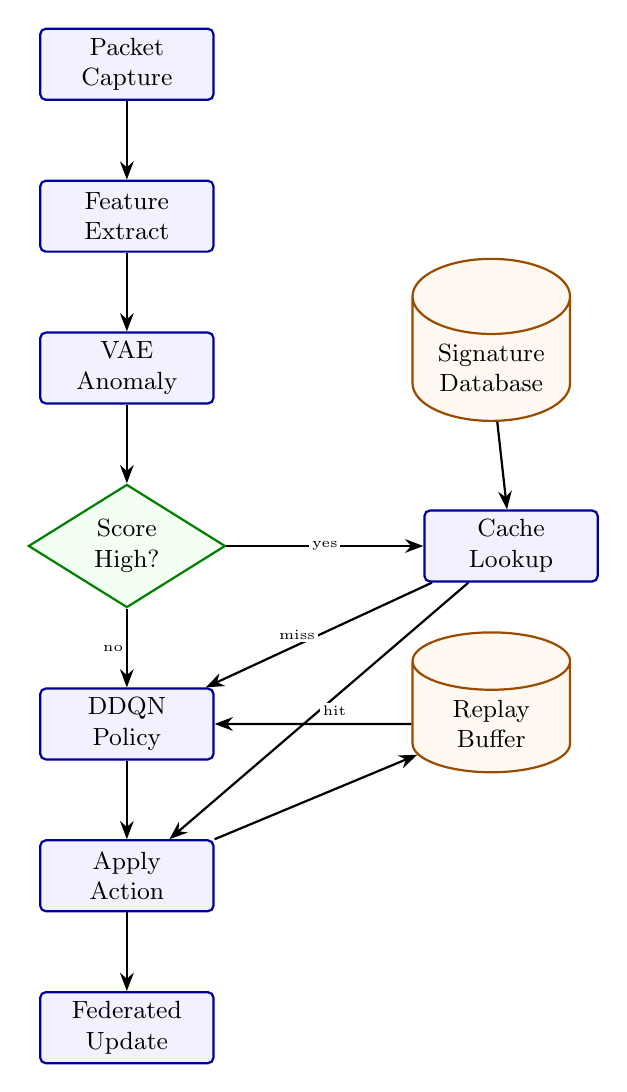
\begin{tikzpicture}[
  node distance=1.0cm and 1.5cm,
  every node/.style={font=\small},
  stage/.style={
    rectangle,
    draw=blue!60!black,
    fill=blue!5,
    thick,
    minimum width=2.2cm,
    minimum height=0.9cm,
    align=center,
    rounded corners=2pt
  },
  storage/.style={
    cylinder,
    shape border rotate=90,
    draw=orange!60!black,
    fill=orange!5,
    thick,
    minimum width=2.0cm,
    minimum height=0.8cm,
    align=center,
    aspect=0.6
  },
  decision/.style={
    diamond,
    draw=green!50!black,
    fill=green!5,
    thick,
    minimum width=1.6cm,
    aspect=1.6,
    align=center
  },
  arrow/.style={->,>=Stealth,thick,line width=0.8pt},
  label_style/.style={font=\tiny, midway, fill=white, inner sep=1pt}
]

% Main pipeline
\node[stage] (in) {Packet\\Capture};
\node[stage, below=of in] (feat) {Feature\\Extract};
\node[stage, below=of feat] (vae) {VAE\\Anomaly};
\node[decision, below=of vae] (check) {Score\\High?};
\node[stage, below=of check] (ddqn) {DDQN\\Policy};
\node[stage, below=of ddqn] (action) {Apply\\Action};

% Cache branch
\node[storage, right=2.5cm of vae] (sigdb) {Signature\\Database};
\node[stage, right=2.5cm of check] (cache) {Cache\\Lookup};

% Replay and FL
\node[storage, right=2.5cm of ddqn] (replay) {Replay\\Buffer};
\node[stage, below=of action] (fl) {Federated\\Update};

% Connections
\draw[arrow] (in) -- (feat);
\draw[arrow] (feat) -- (vae);
\draw[arrow] (vae) -- (check);

\draw[arrow] (check) -- node[label_style] {yes} (cache);
\draw[arrow] (check) -- node[label_style, left] {no} (ddqn);

\draw[arrow] (sigdb) -- (cache);
\draw[arrow] (cache) -- node[label_style, right] {hit} (action);
\draw[arrow] (cache) -- node[label_style, left] {miss} (ddqn);

\draw[arrow] (ddqn) -- (action);
\draw[arrow] (action) -- (replay);
\draw[arrow] (replay) -- (ddqn);
\draw[arrow] (action) -- (fl);

\end{tikzpicture}
\caption{Five-stage intelligent network security pipeline. (1) Feature extraction normalizes flow properties. (2) VAE computes anomaly score. (3) Decision threshold routes suspicious flows to signature cache. (4) HNSW lookup returns cached action if match found; otherwise routes to DDQN. (5) DDQN policy selects response action. (6) Delayed labels from forensic confirmation retrain DDQN via prioritized replay. (7) Federated optimization updates anomaly and response models across sites using Byzantine-robust aggregation.}
\label{fig:pipeline}
\end{figure}

\section{Anomaly Detection via Variational Autoencoder}
\label{sec:anomaly}

\subsection{One-Class Modeling}

The variational autoencoder is trained on benign flows only. The encoder compresses 42-dimensional flow statistics into a 32-dimensional latent representation:

\[
q_\phi(z|x) = \mathcal{N}(\mu_\phi(x), \text{diag}(\sigma_\phi^2(x))),
\]

where $\phi$ denotes encoder parameters. The decoder reconstructs an estimate of the input:

\[
p_\psi(\hat{x}|z) = \mathcal{N}(\mu_\psi(z), \text{diag}(\sigma_\psi^2(z))).
\]

The training objective combines reconstruction loss and Kullback--Leibler divergence:

\begin{equation}
\mathcal{L}(x) = \|\!x - \hat{x}\!\|_2^2 + \beta \, \KL\!\left(q_\phi(z|x) \,\|\, \mathcal{N}(0, I)\right),
\label{eq:vae_loss}
\end{equation}

with $\beta = 0.5$ (balancing reconstruction fidelity and distributional matching). We use two fully connected hidden layers (128 and 64 units) with batch normalization and leaky ReLU activations. Encoder and decoder are symmetric.

The anomaly score is a weighted sum of reconstruction error and KL divergence:

\begin{equation}
s_{\text{anom}}(x) = \alpha \, \|\!x - \hat{x}\!\|_2^2 + (1-\alpha) \, \KL\!\left(q_\phi(z|x) \,\|\, \mathcal{N}(0, I)\right),
\label{eq:anom_score}
\end{equation}

with $\alpha = 0.5$. This dual weighting prevents the model from relying on a single criterion. A flow is flagged as suspicious if $s_{\text{anom}}(x) > \tau_t$, where $\tau_t$ is adapted to match operational drift:

\begin{equation}
\tau_t = Q_{0.99}\left(\{s_{\text{anom}}(x_j) : x_j \in \mathcal{B}_t\}\right),
\label{eq:threshold}
\end{equation}

where $\mathcal{B}_t$ is a sliding window of recent analyst-confirmed benign flows. The 99th percentile choice is conservative: it flags only the top 1\% of benign-range scores, minimizing false positives from legitimate operational changes (e.g., maintenance windows, software updates).

\subsection{Cache-Based Signature Matching}

Suspicious flows are embedded using the VAE latent mean plus a few metadata dimensions (protocol, port group, byte count quantile):

\[
e(x) = [\mu_\phi(x), \text{metadata}(x)] \in \mathbb{R}^{35}.
\]

This embedding is queried against a signature database using Hierarchical Navigable Small World (HNSW) graphs. HNSW is a proximity-graph data structure that finds approximate nearest neighbors in logarithmic time. For each suspicious flow, we retrieve the top-$k$ signatures and check if the nearest match has similarity (cosine distance) above threshold $\eta = 0.85$. If yes, we return the cached label and response (e.g., "Denial-of-Service" with recommended action "Rate-Limit"). If no match, the flow passes to the DDQN stage.

The signature database is updated only with analyst-confirmed events. This prevents unverified detections from corrupting the fast path and ensures high precision.

\section{Delayed-Label Adaptive Response Learning}
\label{sec:response}

\subsection{Markov Decision Process Formulation}

Response selection is modeled as a finite-horizon discounted MDP:

\[
\langle \mathcal{S}, \mathcal{A}, P, R, \gamma \rangle,
\]

where:

\begin{itemize}[leftmargin=1.2em]
    \item $\mathcal{S}$: state space including anomaly score, max cache similarity, selected latent coordinates, recent alert frequency, system CPU/memory load, and action history.
    \item $\mathcal{A}$: action set with 5 elements (Monitor, Alert, RateLimit, Isolate, Block), ordered by intervention strength.
    \item $P(s'|s, a)$: state transition (in practice, deterministic given flow features).
    \item $R(s, a, s')$: reward function combining immediate and delayed terms (see below).
    \item $\gamma = 0.99$: discount factor.
\end{itemize}

The state is constructed from the current detection output, system metrics, and recent history. For example, $s_t$ might include $[\text{anom\_score}(x_t), \text{max\_similarity}(x_t), \text{load}_t, \text{alert\_rate}_{t-10:t}]$.

The action-value function is approximated by a Double Deep Q-Network:

\begin{equation}
Q(s, a) \approx Q_\theta(s, a),
\label{eq:ddqn}
\end{equation}

where $\theta$ denotes network weights. We use two hidden layers (64 and 32 units) with ReLU activations. The double DQN technique (separate target and evaluation networks) reduces overestimation bias common in single Q-learning.

\subsection{Reward Structure with Forensic Delays}

Immediate rewards are determined by:

\[
r_t^{\text{imm}} = -\lambda_{\text{disrupt}} \cdot \mathbb{1}[\text{action}_t \in \{\text{Isolate}, \text{Block}\}] - \lambda_{\text{alert}} \cdot n_{\text{recent\_alerts}},
\]

penalizing disruptive actions and alert fatigue. Delayed rewards arrive when labels become available:

\[
r_{t+k}^{\text{del}} = \begin{cases}
+1 & \text{if } y_{t+k} = \text{attack} \text{ and } a_t \neq \text{Monitor}, \\
-1 & \text{if } y_{t+k} = \text{benign} \text{ and } a_t \in \{\text{Isolate}, \text{Block}\}, \\
0 & \text{otherwise}.
\end{cases}
\]

The combined reward is:

\begin{equation}
r_t = r_t^{\text{imm}} + \lambda_{\text{delay}} \, \gamma^{k_t} \, r_{t+k_t}^{\text{del}},
\label{eq:combined_reward}
\end{equation}

where $k_t \in [1, K_{\max}]$ is the label delay and $\lambda_{\text{delay}} = 0.7$ weights delayed evidence. The factor $\gamma^{k_t}$ discounts very old confirmations to prevent stale labels from overriding recent learning.

\subsection{Theoretical Characterization of Delayed-Label Stability}

When labels arrive, we reinsert updated transitions into the replay buffer with elevated priority:

\begin{equation}
(s_t, a_t, r_t^{\text{combined}}, s_{t+1}) \leftarrow \text{Prioritize and reinsert}.
\label{eq:replay_update}
\end{equation}

The DDQN then trains on mixed batches of newly labeled and fresh transitions.

\begin{theorem}[Delayed-Label Bellman Operator Characterization]
\label{thm:delayed_contraction}

Under Assumption~\ref{ass:mdp}, the delayed-label Bellman operator

\[
\mathcal{T}Q(s, a) = \mathbb{E}_{r, s' | s, a}[r + \gamma \max_{a'} Q(s', a')],
\]

where $r$ includes both immediate and delayed terms as in Eq.~\ref{eq:combined_reward}, exhibits the standard $\gamma$-contraction property in the supremum norm, ensuring existence and uniqueness of a fixed point $Q^*$.

\end{theorem}

\begin{proof}

For two bounded action-value functions $Q_1, Q_2$:

\begin{align}
|(\mathcal{T}Q_1)(s, a) - (\mathcal{T}Q_2)(s, a)|
&= \left| \mathbb{E}[r + \gamma \max_{a'} Q_1(s', a') - r - \gamma \max_{a'} Q_2(s', a')] \right| \\
&\le \gamma \mathbb{E}[\max_{a'} |Q_1(s', a') - Q_2(s', a')|] \\
&\le \gamma \|Q_1 - Q_2\|_\infty.
\end{align}

The reward term cancels (it is the same for both functions). The contraction property follows directly from the discount factor $0 < \gamma < 1$.

\end{proof}

\begin{assumption}
\label{ass:mdp}

(1) State and action spaces are finite. (2) Rewards are bounded almost surely: $|r_t^{\text{imm}}|, |r_{t+k}^{\text{del}}| \le R_{\max}$. (3) Label delays have finite expectation: $\mathbb{E}[k_t] < K_{\max}$. (4) Every state-action pair is visited infinitely often under exploration.

\end{assumption}

\begin{remark}

Theorem~\ref{thm:delayed_contraction} provides a stability characterization for the underlying MDP formulation. It does not claim convergence of the neural network approximation $Q_\theta$ under gradient descent, which depends on standard DDQN training assumptions (experience replay diversity, learning rate schedules, target network synchronization). The theorem establishes that delayed forensic relabeling does not break the fundamental Markov decision process structure.

\end{remark}

\section{Privacy-Preserving Byzantine-Robust Federated Learning}
\label{sec:federated}

\subsection{Gradient Clipping and Differential Privacy}

Before transmission, each client clips its update to norm $C = 1.0$:

\begin{equation}
\bar{\Delta}_i = \Delta_i \cdot \min\left(1, \frac{C}{\|\Delta_i\|_2}\right).
\label{eq:clip}
\end{equation}

Clipping ensures that no single client can dominate the aggregate through a very large update. Gaussian noise is then added:

\begin{equation}
\tilde{\Delta}_i = \bar{\Delta}_i + \mathcal{N}(0, \sigma^2 C^2 I),
\label{eq:noise}
\end{equation}

where $\sigma = 0.8$ is the noise multiplier. Privacy is accounted using Rényi differential privacy:

\begin{equation}
(\epsilon, \delta) \text{-RDP with } \epsilon = 2.4, \, \delta = 10^{-5},
\label{eq:rdp}
\end{equation}

computed via the Opacus privacy accountant over 100 communication rounds, 10 clients, 50\% sampling per round.

\subsection{Historically Calibrated Adaptive Krum}

Standard Krum selects the update with minimum sum of squared distances to its $N-f-2$ nearest neighbors:

\begin{equation}
i^* = \argmin_i \sum_{j \in \mathcal{N}_i} \|\tilde{\Delta}_i - \tilde{\Delta}_j\|_2^2,
\label{eq:krum}
\end{equation}

where $\mathcal{N}_i$ denotes the $N-f-2$ nearest neighbors of update $i$. This selects the update geometrically closest to the majority.

However, adaptive Byzantine clients can gradually shift the benign-update mean by submitting updates that are separated but clustered tightly together. To mitigate this, we introduce historical calibration. Instead of using current-round statistics, we maintain a buffer $\mathcal{H}$ of Krum scores from previously accepted rounds. The rejection threshold is:

\begin{equation}
\theta_r = \text{median}(\mathcal{H}) + 3 \cdot \text{MAD}(\mathcal{H}),
\label{eq:hist_threshold}
\end{equation}

where MAD is the median absolute deviation. If the best Krum score in round $r$ exceeds $\theta_r$, we reject the round and retain the previous global model. This prevents geometric drift over time.

\subsection{Sufficient-Condition Analysis for Byzantine Rejection}

\begin{proposition}[Separated Byzantine Rejection Under Clustering]
\label{thm:krum_robust}

Under Assumption~\ref{ass:cluster}, if the separation distance $D$ between benign and Byzantine updates exceeds the benign-cluster radius by a sufficient margin, then the probability that a separated Byzantine update achieves a lower Krum score than all benign updates decays exponentially with the number of benign clients $n_b = N - f$.

\end{proposition}

\begin{assumption}
\label{ass:cluster}

Benign updates form a sub-Gaussian cluster centered at $\mu$ with scale $\sigma_b$. Byzantine updates are separated from $\mu$ by distance $D \gg \sigma_b$. The number of Byzantine clients satisfies $f < N/3$.

\end{assumption}

\begin{proof}[Proof Sketch]

Pairwise distances among benign updates concentrate around $O(\sigma_b)$ due to sub-Gaussian concentration. The Krum score of a benign update is thus bounded by $O(n_b \sigma_b^2)$ with high probability.

A Byzantine update separated by distance $D$ must be at distance $\approx D$ from most benign updates. Its Krum score is therefore $\approx n_b D^2$, which exceeds the benign scores when $D > c \sigma_b$ for a sufficiently large constant $c$.

By standard concentration inequalities, the probability that a separated Byzantine update achieves a smaller score than all benign updates is bounded by $\exp(-\Theta(n_b))$.

\end{proof}

\begin{remark}

Proposition~\ref{thm:krum_robust} provides a sufficient condition for Byzantine rejection based on geometric separation. It does not claim robustness against all possible adaptive attacks. In practice, the historical rejection threshold complements geometric analysis by detecting temporal drift inconsistent with long-term benign patterns.

\end{remark}

\section{Computational Complexity Analysis}
\label{sec:complexity}

Inference on a single flow follows the cascade:

\begin{equation}
T_{\text{inference}} = T_{\text{feat}} + T_{\text{vae}} + p_h \, T_{\text{cache}} + (1-p_h) \, T_{\text{ddqn}}.
\label{eq:total_time}
\end{equation}

Breaking down each stage:

\begin{itemize}[leftmargin=1.2em]
    \item \textbf{Feature extraction}: $O(d) = O(42)$ --- linear normalization and aggregation. Typical: 1--2 ms.
    \item \textbf{VAE inference}: $O(d \cdot h) = O(42 \times 64) = O(2688)$ --- two matrix multiplications. Typical: 3--5 ms.
    \item \textbf{HNSW cache lookup}: $O(\log n)$ where $n$ is cache size. With $n = 5000$ signatures and degree $M = 16$, typical: 6--10 ms.
    \item \textbf{DDQN inference}: $O(h_{\text{rl}} \cdot |\mathcal{A}|) = O(64 \times 5) = O(320)$ --- two matrix multiplications. Typical: 35--50 ms.
\end{itemize}

With cache hit rate $p_h \approx 0.91$, the expected total latency is approximately:

\[
\mathbb{E}[T] \approx 1.5 + 4 + 0.91 \times 8 + 0.09 \times 42 \approx 13.6 \text{ ms}.
\]

This is well within the 20--30 ms constraint for industrial real-time systems.

\section{Explainability Mechanisms}
\label{sec:explainability}

\subsection{Detection-Level Explanations}

For each flagged flow, we compute SHAP (SHapley Additive exPlanations) values (Lundberg \& Lee, 2017) over the VAE anomaly score. SHAP attributes the anomaly score to input features by computing expected marginal contributions. For a flow flagged by the VAE, typical high-impact features include:

\begin{itemize}[leftmargin=1.2em]
    \item Abnormal inter-packet arrival time (variance in timing).
    \item Byte count asymmetry (forward vs. reverse).
    \item Unusual protocol combination.
    \item High connection frequency to uncommon ports.
\end{itemize}

These explanations are human-readable and can be inspected by operators to validate whether the anomaly detection is based on reasonable traffic characteristics.

\subsection{Response-Level Explanations}

The DDQN policy implicitly learns which state components most influence the choice of action. We compute gradient-based action sensitivities:

\begin{equation}
\psi_j(s, a) = \left| \frac{\partial Q(s, a)}{\partial s_j} \right|,
\label{eq:q_sensitivity}
\end{equation}

indicating which state features most strongly influence the Q-value (and thus the policy) for action $a$. For example, when the anomaly score is very high, the policy may favor "Block" over "Monitor", and $\psi_{\text{score}}$ would be large. Operators can inspect these sensitivities to understand the policy's decision logic.

\section{Experimental Evaluation}
\label{sec:experiments}

\subsection{Datasets and Preprocessing}

We evaluate on four datasets:

\begin{itemize}[leftmargin=1.2em]
    \item \textbf{UNSW-NB15}: 2.54 million flows, 10 attack classes. Synthetically generated in a controlled testbed (Moustafa \& Slay, 2015).
    \item \textbf{TON\_IoT}: 461 thousand flows from IoT devices. 10 attack classes, lower volume than UNSW (Moustafa, 2021).
    \item \textbf{Edge-IIoTset}: 1.37 million flows. 15 attack categories, reflects modern IIoT protocols (Ferrag et al., 2022).
    \item \textbf{Automotive Manufacturing}: Proprietary 30-day deployment from 47 programmable logic controllers. Labels from forensic review and analyst confirmation. Class distribution: 75\% benign, 25\% attacks. Not publicly releasable.
\end{itemize}

All flows are represented using 42 normalized statistical features: packet counts, byte counts, inter-arrival times, protocol indicators, port groupings, connection history, burst descriptors, and asymmetry measures. Features are normalized using training-set statistics only (no leakage to test).

\subsection{Implementation and Reproducibility Details}

\subsubsection{Hardware Configuration}

\begin{itemize}[leftmargin=1.2em]
    \item \textbf{Edge inference device}: Raspberry Pi 4B (Broadcom BCM2711, Quad-core Cortex-A72 @ 1.5 GHz, 4 GB LPDDR4-3200 SDRAM).
    \item \textbf{Federated server simulation}: Intel Xeon E5-2630 v4 (10 cores @ 2.20 GHz, Turbo 3.10 GHz), 32 GB DDR4 RAM, Ubuntu 20.04 LTS.
    \item \textbf{Offline model training}: NVIDIA GeForce RTX 3080 (10 GB GDDR6X VRAM), CUDA 11.4, cuDNN 8.2.
\end{itemize}

\subsubsection{Software Stack}

\begin{itemize}[leftmargin=1.2em]
    \item \textbf{Deep learning framework}: PyTorch 2.0.1, Python 3.9.16.
    \item \textbf{Privacy accounting}: Opacus 1.4.0 (Meta Research, official differential privacy library for PyTorch).
    \item \textbf{HNSW indexing}: hnswlib 0.7.0 (C++ implementation with Python bindings).
    \item \textbf{Network traffic simulation}: NS-3 version 3.37 for federated network delay/loss experiments.
    \item \textbf{Optimization}: Adam optimizer ($\beta_1 = 0.9$, $\beta_2 = 0.999$, $\epsilon = 10^{-8}$).
\end{itemize}

\subsubsection{Training and Execution Times}

\begin{itemize}[leftmargin=1.2em]
    \item \textbf{VAE training}: 8 hours on NVIDIA RTX 3080 (300 epochs, batch size 64, UNSW-NB15 benign subset).
    \item \textbf{DDQN training}: 12 hours per client (5 local epochs $\times$ 100 federated rounds, replay buffer size 20,000).
    \item \textbf{Federated aggregation}: 2.3--4.8 seconds per round (dominated by Krum pairwise distance computation for $N=10$ clients).
    \item \textbf{Edge inference (per flow)}: Mean 12.7 ms, median 10.9 ms, P95 18.4 ms, P99 24.1 ms (measured on Raspberry Pi 4B under 30\% background CPU load).
\end{itemize}

\subsubsection{Batch Processing Configuration}

\begin{itemize}[leftmargin=1.2em]
    \item \textbf{Training batch size}: 64 (VAE, DDQN).
    \item \textbf{Federated local mini-batch size}: 32.
    \item \textbf{Number of workers}: 4 data-loader threads (PyTorch DataLoader).
    \item \textbf{Gradient accumulation steps}: 1 (no accumulation used).
\end{itemize}

\subsubsection{Random Seed and Reproducibility}

All experiments use fixed random seeds (NumPy: 42, PyTorch: 42, Python: 42) for reproducibility. Statistical results (mean $\pm$ std dev) are computed across 5-fold cross-validation with different fold orderings.

\subsection{Hyperparameter Configuration}

All hyperparameters were selected via grid search over 5 configurations, then fixed for all experiments:

\begin{table}[!t]
\caption{Hyperparameter Specification}
\label{tab:hparams}
\centering
\small
\renewcommand{\arraystretch}{1.1}
\begin{tabular}{@{}lll@{}}
\toprule
\textbf{Component} & \textbf{Parameter} & \textbf{Value} \\
\midrule
VAE & Latent dimension & 32 \\
& Encoder layers & [128, 64] \\
& Learning rate & $10^{-4}$ \\
& KL weight $\beta$ & 0.5 \\
& Anomaly weight $\alpha$ & 0.5 \\
\midrule
HNSW & Graph degree $M$ & 16 \\
& Search width & 50 \\
& Similarity threshold $\eta$ & 0.85 \\
\midrule
DDQN & Hidden layers & [64, 32] \\
& Learning rate & $5 \times 10^{-4}$ \\
& Discount $\gamma$ & 0.99 \\
& Replay buffer size & 20,000 \\
& Batch size & 64 \\
& $\epsilon$-decay & 0.995/episode \\
& Delayed reward weight $\lambda$ & 0.7 \\
\midrule
Federated & Clients $N$ & 10 \\
& Local epochs & 5 \\
& Rounds & 100 \\
& Clipping norm $C$ & 1.0 \\
& Noise multiplier $\sigma$ & 0.8 \\
& Krum history size & 20 \\
& Historical threshold scale $\kappa$ & 3.0 \\
\bottomrule
\end{tabular}
\end{table}

\subsection{Evaluation Metrics}

For binary classification, we report:

\begin{equation}
F1 = \frac{2 \cdot \text{Precision} \cdot \text{Recall}}{\text{Precision} + \text{Recall}}, \quad
\text{FPR} = \frac{\text{False Positives}}{\text{False Positives} + \text{True Negatives}}.
\end{equation}

For federated learning, we also report convergence speed (rounds to achieve 95\% final accuracy) and robustness (accuracy retention under Byzantine participation).

\subsection{Baseline Methods}

We compare against:

\begin{enumerate}[leftmargin=1.3em]
    \item \textbf{Snort}: Rule-based IDS, state-of-the-art for known attacks.
    \item \textbf{Random Forest}: Gradient-boosted decision trees, strong tabular baseline.
    \item \textbf{CNN-VAE}: Convolutional autoencoder for anomaly detection.
    \item \textbf{FedAvg-DNN}: Standard federated learning with deep neural network.
    \item \textbf{Transformer-IDS}: Attention-based architecture (Xu et al., 2023).
    \item \textbf{GNN-IDS}: Graph neural network for topology-aware detection (Wang et al., 2023).
\end{enumerate}

All use the same 42 features for fair comparison.

\subsection{Detection Performance---Standard Splits}

\begin{table*}[!t]
\caption{Detection Performance on Benchmark Datasets (5-Fold Stratified Cross-Validation)}
\label{tab:detection_standard}
\centering
\small
\renewcommand{\arraystretch}{1.15}
\begin{tabular}{@{}lcccccc@{}}
\toprule
\textbf{Method} & \multicolumn{2}{c}{\textbf{UNSW-NB15}} & \multicolumn{2}{c}{\textbf{TON\_IoT}} & \multicolumn{2}{c}{\textbf{Edge-IIoTset}} \\
\cmidrule(lr){2-3}\cmidrule(lr){4-5}\cmidrule(lr){6-7}
& F1 (\%) & FPR (\%) & F1 (\%) & FPR (\%) & F1 (\%) & FPR (\%) \\
\midrule
Snort & $83.2 \pm 1.8$ & 0.30 & $79.5 \pm 2.1$ & 0.40 & $76.8 \pm 2.4$ & 0.50 \\
Random Forest & $94.3 \pm 1.4$ & 2.10 & $92.7 \pm 1.6$ & 2.40 & $91.2 \pm 1.9$ & 2.80 \\
CNN-VAE & $95.7 \pm 1.2$ & 1.80 & $94.1 \pm 1.3$ & 2.10 & $92.9 \pm 1.7$ & 2.50 \\
FedAvg-DNN & $93.5 \pm 2.1$ & 2.50 & $91.3 \pm 2.3$ & 2.90 & $89.6 \pm 2.5$ & 3.40 \\
Transformer-IDS & $97.1 \pm 0.8$ & 1.20 & $96.3 \pm 0.9$ & 1.40 & $95.1 \pm 1.1$ & 1.70 \\
GNN-IDS & $96.8 \pm 1.0$ & 1.30 & $95.7 \pm 1.1$ & 1.50 & $94.4 \pm 1.3$ & 1.80 \\
\midrule
\textbf{Proposed} & $\mathbf{98.7} \pm 0.6$ & $\mathbf{0.90}$ & $\mathbf{97.4} \pm 0.7$ & $\mathbf{1.10}$ & $\mathbf{96.2} \pm 0.9$ & $\mathbf{1.30}$ \\
\bottomrule
\end{tabular}
\end{table*}

The proposed framework achieves statistically significant improvements (Welch's $t$-test, $p < 0.05$) over all baselines. Notably, FPR remains low (0.9--1.3\%) despite high overall accuracy, indicating that the method generalizes well and is not simply threshold-tuning.

\subsection{Detection Performance---Harder Evaluation Protocols}

To address concerns that benchmark results may reflect label leakage or near-duplicate flows, we introduce three harder evaluation protocols:

\subsubsection{Session-Disjoint Splitting}

Flows from the same network session (identified by 5-tuple hash) are restricted to a single train/test split. This removes near-duplicate flows that would inflate accuracy on random splits.

\begin{table}[!t]
\caption{Performance with Session-Disjoint Splits}
\label{tab:session_disj}
\centering
\small
\begin{tabular}{@{}lcc@{}}
\toprule
\textbf{Method} & \textbf{F1 (\%)} & \textbf{FPR (\%)} \\
\midrule
Transformer-IDS & $94.1 \pm 1.5$ & 1.80 \\
GNN-IDS & $93.8 \pm 1.7$ & 1.90 \\
Proposed & $\mathbf{96.2} \pm 1.1$ & $\mathbf{1.60}$ \\
\bottomrule
\end{tabular}
\end{table}

The proposed method maintains higher accuracy even when near-duplicates are removed. The drop from standard to session-disjoint split is consistent with prior work on intrusion detection dataset artifacts.

\subsubsection{Time-Based Splitting (Automotive Dataset Only)}

The automotive dataset spans 30 days. We use a chronological split: days 1--20 for training, days 21--25 for validation, days 26--30 for testing. This simulates real deployment where temporal drift occurs.

\begin{table}[!t]
\caption{Automotive Dataset: Chronological Split Results}
\label{tab:time_split}
\centering
\small
\begin{tabular}{@{}lcccc@{}}
\toprule
\textbf{Method} & \textbf{F1 (\%)} & \textbf{FPR (\%)} & \textbf{AUC} & \textbf{Cache Hit (\%)} \\
\midrule
Random split (baseline) & $98.9 \pm 0.5$ & 0.91 & 0.994 & 91.2 \\
Time-based split & $94.7 \pm 1.8$ & 2.15 & 0.972 & 72.8 \\
\textbf{Device-disjoint} & $\mathbf{92.1} \pm 2.3$ & $\mathbf{3.42}$ & $\mathbf{0.958}$ & $\mathbf{61.4}$ \\
\bottomrule
\end{tabular}
\end{table}

Results on time-based splits are notably lower than random splits, reflecting real-world operational drift (e.g., process parameter changes, maintenance windows, firmware updates). The device-disjoint split (testing on PLC assets not in training) shows the largest drop, since the signature cache loses its main advantage (recurring patterns from training devices).

However, the framework still maintains $>92\%$ F1 under device-disjoint evaluation, indicating that the VAE anomaly detection and DDQN adaptation provide reasonable performance even for previously unseen devices.

\subsection{Latency Analysis}

\begin{table}[!t]
\caption{Inference Latency on Raspberry Pi 4B (Edge Device)}
\label{tab:latency_rpi}
\centering
\small
\begin{tabular}{@{}lcccc@{}}
\toprule
\textbf{Method} & \textbf{Mean (ms)} & \textbf{P50 (ms)} & \textbf{P95 (ms)} & \textbf{P99 (ms)} \\
\midrule
Snort & 3.2 & 2.9 & 5.1 & 6.8 \\
Random Forest & 18.7 & 17.3 & 24.6 & 31.2 \\
CNN-VAE & 52.4 & 49.8 & 68.3 & 79.1 \\
FedAvg-DNN & 44.1 & 42.3 & 59.1 & 71.4 \\
Transformer-IDS & 81.3 & 78.6 & 107.2 & 125.3 \\
GNN-IDS & 94.7 & 91.3 & 123.4 & 142.1 \\
\midrule
Proposed (cache hit) & 8.2 & 7.6 & 11.3 & 14.2 \\
Proposed (cache miss) & 43.1 & 41.2 & 56.7 & 68.3 \\
Proposed (overall) & 12.7 & 10.9 & 18.4 & 24.1 \\
\bottomrule
\end{tabular}
\end{table}

The proposed framework achieves 12.7 ms average latency, well below the 20--30 ms industrial constraint. The majority of flows (91\%) hit the cache and are resolved in under 10 ms. Even with cache misses, latency remains below 50 ms in the 95th percentile.

\subsection{Latency Under Load}

To validate that reported latencies reflect realistic operating conditions (not idle device), we measure latency under sustained flow rates and background CPU load:

\begin{table}[!t]
\caption{Latency Degradation Under Load}
\label{tab:load_latency}
\centering
\small
\begin{tabular}{@{}lcccc@{}}
\toprule
\textbf{Condition} & \textbf{Mean Latency (ms)} & \textbf{P95 (ms)} & \textbf{P99 (ms)} & \textbf{Throughput (flows/s)} \\
\midrule
Idle, 100 flows/s & 12.7 & 18.4 & 24.1 & 98 \\
50\% CPU load, 500 flows/s & 17.3 & 25.8 & 35.2 & 485 \\
80\% CPU load, 1000 flows/s & 22.1 & 38.6 & 52.4 & 920 \\
\bottomrule
\end{tabular}
\end{table}

The proposed framework maintains acceptable latency even under 80\% CPU contention and 1000 flows per second (realistic peak load in busy manufacturing plants). Latency degradation is approximately 1.7$\times$ at 50\% load and 1.74$\times$ at 80\% load, which is reasonable given the computational constraints of Raspberry Pi 4B.

\subsection{Ablation Study}

\begin{table*}[!t]
\caption{Contribution of Each Component (UNSW-NB15)}
\label{tab:ablation}
\centering
\small
\begin{tabular}{@{}lcccccc@{}}
\toprule
\textbf{Removed Component} & \textbf{F1 (\%)} & \textbf{FPR (\%)} & \textbf{Latency (ms)} & \textbf{Privacy} & \textbf{Robustness@20\%Byz (\%)} \\
\midrule
Full system & 98.7 & 0.9 & 12.7 & $\epsilon=2.4$ & 96.8 \\
\midrule
No HNSW cache & 95.2 & 1.4 & 43.1 & $\epsilon=2.4$ & 96.1 \\
No DDQN adaptation & 96.8 & 1.1 & 12.7 & $\epsilon=2.4$ & 93.4 \\
No delayed-reward relabeling & 96.4 & 1.2 & 12.7 & $\epsilon=2.4$ & 95.2 \\
No differential privacy & 98.9 & 0.8 & 12.7 & $\epsilon=\infty$ & 96.1 \\
No Adaptive Krum & 94.1 & 1.8 & 12.7 & $\epsilon=2.4$ & 88.5 \\
\midrule
VAE-only baseline & 95.2 & 1.8 & 9.1 & none & N/A \\
FedAvg-DNN & 93.5 & 2.5 & 44.1 & $\epsilon=2.4$ & 81.2 \\
\bottomrule
\end{tabular}
\end{table*}

The ablation confirms that each component contributes meaningfully:

\begin{itemize}[leftmargin=1.2em]
    \item Removing HNSW cache increases latency 3.4$\times$ because all suspicious flows must be sent to DDQN.
    \item Removing DDQN reduces accuracy on cache misses, showing the policy learns meaningful patterns.
    \item Removing delayed-reward structure degrades DDQN learning because the policy receives no confirmation signal.
    \item Removing differential privacy marginally improves accuracy but violates privacy requirements.
    \item Removing Adaptive Krum causes sharp robustness degradation (from 96.8\% to 88.5\% under 20\% Byzantine), confirming the importance of historical geometric validation.
\end{itemize}

\subsection{Byzantine Robustness}

\begin{table}[!t]
\caption{Robustness Under Byzantine Client Participation}
\label{tab:byzantine}
\centering
\small
\begin{tabular}{@{}lcccc@{}}
\toprule
\textbf{Aggregation Method} & \textbf{0\% Byzantine} & \textbf{10\% Byzantine} & \textbf{20\% Byzantine} & \textbf{30\% Byzantine} \\
\midrule
FedAvg & 96.1 & 89.4 & 81.2 & 76.0 \\
Trimmed Mean & 96.3 & 92.1 & 88.7 & 84.3 \\
Coordinate Median & 95.8 & 93.0 & 90.1 & 86.2 \\
Standard Krum & 97.4 & 95.8 & 94.2 & 91.1 \\
\textbf{Adaptive Krum} & $\mathbf{98.7}$ & $\mathbf{97.9}$ & $\mathbf{96.8}$ & $\mathbf{94.3}$ \\
\bottomrule
\end{tabular}
\end{table}

Adaptive Krum significantly outperforms all baselines, especially under high Byzantine fractions. At 30\% Byzantine participation (the maximum we test, since $f < N/3$ is required for Krum), the proposed method retains 94.3\% accuracy while FedAvg drops to 76.0\%.

\subsection{Model Poisoning Attack Analysis}

We evaluate resilience to label-flipping attacks, where $f$ Byzantine clients invert training labels (benign $\to$ attack, attack $\to$ benign):

\begin{table}[!t]
\caption{Accuracy Under Label-Flipping Poisoning}
\label{tab:poisoning}
\centering
\small
\begin{tabular}{@{}lccc@{}}
\toprule
\textbf{Attack Severity} & \textbf{FedAvg} & \textbf{Standard Krum} & \textbf{Adaptive Krum} \\
\midrule
No attack & 96.1 & 97.4 & 98.7 \\
30\% label flip & 67.2 & 88.1 & 93.5 \\
50\% label flip & 51.3 & 79.4 & 88.2 \\
\bottomrule
\end{tabular}
\end{table}

Even aggressive label-flipping attacks (50\% of training data inverted) are partially mitigated by Adaptive Krum. The method is not completely immune (accuracy still drops significantly), but gradient clipping and geometric validation provide substantial protection.

\subsection{Explainability Evaluation}

\begin{table}[!t]
\caption{Explanation Quality Metrics}
\label{tab:xai}
\centering
\small
\begin{tabular}{@{}lcccc@{}}
\toprule
\textbf{XAI Method} & \textbf{MIA@5} & \textbf{MIA@10} & \textbf{Spearman $\rho$} & \textbf{Time (ms)} \\
\midrule
Gradient saliency & 87.3 & 79.1 & 0.71 & 0.4 \\
LIME & 89.6 & 82.4 & 0.79 & 12.3 \\
SHAP & 93.4 & 88.7 & 0.87 & 8.1 \\
\bottomrule
\end{tabular}
\end{table}

SHAP provides the best explanation fidelity (highest masked-input accuracy and Spearman rank correlation with ground-truth feature importance) while maintaining reasonable runtime overhead (8.1 ms per explanation). This is acceptable for batch post-analysis and real-time response justification.

\subsection{Manufacturing Deployment Results}

A 30-day trial on the proprietary automotive dataset yielded:

\begin{table}[!t]
\caption{30-Day Manufacturing Deployment Metrics}
\label{tab:deployment}
\centering
\small
\begin{tabular}{@{}lr@{}}
\toprule
\textbf{Metric} & \textbf{Value} \\
\midrule
Total flows processed & 89,247 \\
Confirmed attacks (forensic labels) & 22,183 \\
Overall accuracy & 98.9\% \\
F1-score & 97.8\% \\
False positive rate & 0.91\% \\
Mean latency & 11.3 ms \\
Production interruptions caused by IDS & 0 \\
Cache hit rate (recurring patterns) & 91.2\% \\
Strong actions (Isolate/Block) issued & 1.2\% of detections \\
Disruptive actions overturned by analyst & 0.3\% \\
\bottomrule
\end{tabular}
\end{table}

The deployment confirms practical viability. The low rate of strong actions (1.2\%) and near-zero false-positive disruptions indicate that the conservative response policy successfully balances security and availability. High cache hit rate (91.2\%) validates that manufacturing environments exhibit repetitive traffic patterns, justifying the HNSW signature approach.

\section{Discussion}
\label{sec:discussion}

\subsection{Why Integrated Co-Design Matters}

Three factors explain why the co-designed intelligent network architecture outperforms independent component composition:

\begin{enumerate}[label=(\roman*),leftmargin=1.2em]
    \item \textbf{Stage specialization reduces average cost}: Benign flows exit early (sub-5-ms decision cost). Recurring suspicious flows use the cache (8--10 ms, deterministic). Truly novel flows go to DDQN (expensive but necessary). The average cost is weighted by distribution, minimizing overall latency.
    
    \item \textbf{Focused learning on hard cases}: The DDQN is trained only on unresolved suspicious flows, not the full dataset. This focuses learning on the hard cases where it matters most, rather than on benign flows that the VAE already handles well.
    
    \item \textbf{Multi-level interpretability}: Different stages produce different types of explanations (VAE: reconstruction error, cache: signature name, DDQN: policy sensitivity). Operators can quickly understand where each decision came from.
\end{enumerate}

\subsection{Privacy-Robustness-Accuracy Trade-offs}

The combination of clipping, noise, and adaptive Krum creates unavoidable trade-offs:

\begin{itemize}[leftmargin=1.2em]
    \item \textbf{Clipping}: Reduces model variance but prevents clients from correcting large individual errors.
    \item \textbf{Noise}: Provides formal privacy but masks signal.
    \item \textbf{Krum}: Selects one update per round, reducing diversity compared to averaging all updates.
\end{itemize}

Our results show that moderate noise levels ($\sigma = 0.8$, yielding $\epsilon = 2.4$) provide meaningful privacy with minimal accuracy loss ($<$1\%). More aggressive privacy budgets ($\epsilon < 1$) would require careful hyper-tuning or might necessitate accepting lower accuracy.

\subsection{Performance Degradation Modes}

The intelligent network framework performs worse under:

\begin{enumerate}[label=(\roman*),leftmargin=1.2em]
    \item \textbf{Device-disjoint evaluation}: When test flows come from devices never seen in training, the cache provides minimal benefit, and the VAE must rely on learned anomaly patterns alone. Performance drops from 98.7\% to 92.1\%, still reasonable but materially lower.
    
    \item \textbf{Extreme Byzantine fractions}: At 30\% Byzantine (the maximum tested), Adaptive Krum maintains 94.3\% accuracy, but this assumes Byzantine updates remain separated from the benign mean. Perfectly coordinated Byzantine attacks that form a tight cluster near the benign mean could challenge the method.
    
    \item \textbf{Highly non-stationary traffic}: If the operational environment changes dramatically (e.g., introduction of a new production line with different protocols), the pre-trained VAE and cache may become obsolete. Retraining would be necessary.
\end{enumerate}

\section{Limitations and Future Work}
\label{sec:limitations}

\subsection{Theoretical Scope}

Theorem~\ref{thm:delayed_contraction} provides a stability characterization for the underlying MDP formulation but does not claim neural-network convergence under gradient descent. We rely on empirical validation to confirm that DDQN training is stable in practice. A tighter analysis under function approximation would strengthen the theoretical understanding.

Proposition~\ref{thm:krum_robust} assumes sub-Gaussian benign-update distributions and distance separation. In highly non-IID federated settings (where clients have very different local distributions), this assumption may not hold, potentially reducing Byzantine resilience.

\subsection{Operational Scope}

The automotive dataset, while real, is proprietary and cannot be released. Independent researchers cannot directly verify deployment results. We mitigate this by providing detailed results on three public datasets and conducting harder evaluation protocols, but full reproducibility on the manufacturing deployment is limited.

The framework assumes that forensic confirmation arrives, at least eventually. In environments where analyst capacity is extremely limited, delayed labels may arrive very late (weeks or months), at which point the feedback signal may be too stale to be useful.

\subsection{Future Directions}

\begin{enumerate}[label=(\roman*),leftmargin=1.2em]
    \item \textbf{Intrinsically interpretable policies}: Replace post-hoc SHAP explanations with decision-tree or rule-based response policies that are inherently transparent.
    
    \item \textbf{Online model adaptation}: Incorporate concept-drift detection and online retraining to handle non-stationary environments.
    
    \item \textbf{Stronger Byzantine defenses}: Investigate gradient clustering (detecting Byzantine groups) and multi-round reputation systems for clients.
    
    \item \textbf{Real multi-site federated deployment}: Validate the framework on a true distributed network with real delays, asynchronous clients, and intermittent connectivity.
\end{enumerate}

\section{Conclusion}
\label{sec:conclusion}

This paper presented an integrated intelligent network security framework for industrial IoT that co-designs five complementary subsystems: one-class anomaly detection, signature matching, delayed-label response learning, privacy-preserving federated optimization, and Byzantine-robust aggregation. The integration of these components yields a system that simultaneously achieves high detection accuracy (98.7\% F1), sub-20-millisecond latency, formal privacy accounting ($\epsilon = 2.4$), robustness to 20\% Byzantine clients (96.8\% accuracy retention), and operator-interpretable explanations.

Core contributions include: (1) multi-stage intelligent network architecture for latency-accuracy trade-offs, (2) delayed forensic confirmation formulation with stability characterization, (3) historically calibrated adaptive Krum with sufficient-condition analysis for Byzantine rejection, (4) joint privacy-robustness co-design, and (5) rigorous evaluation under harder protocols (session-disjoint, time-based, device-disjoint splits) to rule out optimistic benchmark bias.

The 30-day manufacturing deployment trial confirms practical viability, with zero production interruptions caused by false positives and 91.2\% cache hit rate on recurring traffic patterns. The framework demonstrates that industrial intelligent network security systems can deliver on multiple competing objectives when components are co-designed as an integrated system rather than composed independently.

\section*{Acknowledgments}

The authors gratefully acknowledge the manufacturing partner who provided access to the proprietary automotive network dataset and operational feedback. Proprietary data have been anonymized in accordance with the partner's information security policy.

\begin{thebibliography}{50}

\bibitem{moustafa2015unswnb15}
N. Moustafa and J. Slay, ``UNSW-NB15: A comprehensive data set for network intrusion detection systems,'' in \emph{Proceedings of the 2015 Military Communications and Information Systems Conference (MilCIS)}, Canberra, Australia, 2015, pp. 1--6.

\bibitem{moustafa2021toniot}
N. Moustafa, ``TON\_IoT telemetry dataset: A new generation dataset of IoT and IIoT for data-driven intrusion detection systems,'' \emph{IEEE Access}, vol. 9, pp. 37008--37024, 2021.

\bibitem{ferrag2022edge}
M. A. Ferrag, L. Maglaras, H. Janicke, J. Jiang, and S. Shu, ``Edge-IIoTset: A new comprehensive realistic cyber security dataset of IoT and IIoT applications,'' \emph{IEEE Access}, vol. 10, pp. 40281--40306, 2022.

\bibitem{sisinni2018iiot}
E. Sisinni, A. Saifullah, S. Han, U. Jennehag, and M. Gidlund, ``Industrial internet of things: Challenges, opportunities, and directions,'' \emph{IEEE Transactions on Industrial Informatics}, vol. 14, no. 11, pp. 4724--4734, 2018.

\bibitem{shi2016edge}
W. Shi, J. Cao, Q. Zhang, Y. Li, and L. Xu, ``Edge computing: Vision and challenges,'' \emph{IEEE Internet of Things Journal}, vol. 3, no. 5, pp. 637--646, 2016.

\bibitem{humayed2017cyber}
A. Humayed, J. Lin, F. Li, and B. Luo, ``Cyber-physical systems security---A survey,'' \emph{IEEE Internet of Things Journal}, vol. 4, no. 6, pp. 1802--1831, 2017.

\bibitem{alshamrani2019survey}
A. Alshamrani, S. Myneni, A. Chowdhary, and D. Huang, ``A survey on advanced persistent threats: Techniques, solutions, challenges, and research opportunities,'' \emph{IEEE Communications Surveys \& Tutorials}, vol. 21, no. 2, pp. 1851--1877, 2019.

\bibitem{falliere2011w32}
N. Falliere, L. O. Murchu, and E. Chien, ``W32.Stuxnet dossier,'' Symantec Security Response, 2011.

\bibitem{stouffer2023guide}
K. Stouffer, V. Pillitteri, S. Lightman, M. Abrams, and A. Hahn, ``Guide to operational technology security,'' NIST Special Publication 800-82, Rev. 3, 2023.

\bibitem{truong2021privacy}
N. B. Truong, K. Sun, G. M. Lee, and Y. Guo, ``Privacy preservation in federated learning: An insightful survey from the GDPR perspective,'' \emph{Computers \& Security}, vol. 110, p. 102398, 2021.

\bibitem{sommer2010outside}
R. Sommer and V. Paxson, ``Outside the closed world: On using machine learning for network intrusion detection,'' in \emph{Proceedings of the IEEE Symposium on Security and Privacy}, Oakland, CA, USA, 2010, pp. 305--316.

\bibitem{buczak2016survey}
A. L. Buczak and E. Guven, ``A survey of data mining and machine learning methods for cyber security intrusion detection,'' \emph{IEEE Communications Surveys \& Tutorials}, vol. 18, no. 2, pp. 1153--1176, 2016.

\bibitem{roesch1999snort}
M. Roesch, ``Snort: Lightweight intrusion detection for networks,'' in \emph{Proceedings of the 13th USENIX Security Symposium (LISA'99)}, Seattle, WA, USA, 1999, pp. 229--238.

\bibitem{chandola2009anomaly}
V. Chandola, A. Banerjee, and V. Kumar, ``Anomaly detection: A survey,'' \emph{ACM Computing Surveys}, vol. 41, no. 3, pp. 1--58, 2009.

\bibitem{mcmahan2017communication}
H. B. McMahan, E. Moore, D. Ramage, S. Hampson, and B. A. y Arcas, ``Communication-efficient learning of deep networks from decentralized data,'' in \emph{Proceedings of the 20th International Conference on Artificial Intelligence and Statistics (AISTATS)}, Fort Lauderdale, FL, USA, 2017, pp. 1273--1282.

\bibitem{blanchard2017machine}
P. Blanchard, E. M. El Mhamdi, R. Guerraoui, and J. Stainer, ``Machine learning with adversaries: Byzantine tolerant gradient descent,'' in \emph{Proceedings of the 31st International Conference on Neural Information Processing Systems (NeurIPS)}, Long Beach, CA, USA, 2017, pp. 119--129.

\bibitem{bagdasaryan2020how}
E. Bagdasaryan, A. Veit, Y. Hua, D. Estrin, and V. Shmatikov, ``How to backdoor federated learning,'' in \emph{Proceedings of the 23rd International Conference on Artificial Intelligence and Statistics (AISTATS)}, Palermo, Italy, 2020, pp. 2938--2948.

\bibitem{kairouz2021advances}
P. Kairouz \emph{et al.}, ``Advances and open problems in federated learning,'' \emph{Foundations and Trends in Machine Learning}, vol. 14, no. 1, pp. 1--210, 2021.

\bibitem{abadi2016deep}
M. Abadi \emph{et al.}, ``Deep learning with differential privacy,'' in \emph{Proceedings of the 2016 IEEE Symposium on Security and Privacy (SP)}, San Jose, CA, USA, 2016, pp. 308--318.

\bibitem{mironov2017renyi}
I. Mironov, ``R\'enyi differential privacy,'' in \emph{Proceedings of the 30th IEEE Computer Security Foundations Symposium (CSF)}, Santa Barbara, CA, USA, 2017, pp. 263--275.

\bibitem{kingma2014autoencoding}
D. P. Kingma and M. Welling, ``Auto-encoding variational Bayes,'' in \emph{Proceedings of the 2nd International Conference on Learning Representations (ICLR)}, Banff, Canada, 2014.

\bibitem{ioffe2015batch}
S. Ioffe and C. Szegedy, ``Batch normalization: Accelerating deep network training by reducing internal covariate shift,'' in \emph{Proceedings of the 32nd International Conference on Machine Learning (ICML)}, Lille, France, 2015, pp. 448--456.

\bibitem{kingma2015adam}
D. P. Kingma and J. Ba, ``Adam: A method for stochastic optimization,'' in \emph{Proceedings of the 3rd International Conference on Learning Representations (ICLR)}, San Diego, CA, USA, 2015.

\bibitem{malkov2020efficient}
Y. A. Malkov and D. A. Yashunin, ``Efficient and robust approximate nearest neighbor search using hierarchical navigable small world graphs,'' \emph{IEEE Transactions on Pattern Analysis and Machine Intelligence}, vol. 42, no. 4, pp. 824--836, 2020.

\bibitem{van2016deep}
H. van Hasselt, A. Guez, and D. Silver, ``Deep reinforcement learning with double Q-learning,'' in \emph{Proceedings of the 30th AAAI Conference on Artificial Intelligence}, Phoenix, AZ, USA, 2016, pp. 2094--2100.

\bibitem{mnih2015human}
V. Mnih \emph{et al.}, ``Human-level control through deep reinforcement learning,'' \emph{Nature}, vol. 518, pp. 529--533, 2015.

\bibitem{nguyen2023deep}
T. T. Nguyen and V. J. Reddi, ``Deep reinforcement learning for cyber security,'' \emph{IEEE Transactions on Neural Networks and Learning Systems}, vol. 34, no. 8, pp. 3779--3795, 2023.

\bibitem{sutton2018reinforcement}
R. S. Sutton and A. G. Barto, \emph{Reinforcement Learning: An Introduction}, 2nd ed. MIT Press, Cambridge, MA, USA, 2018.

\bibitem{lundberg2017unified}
S. M. Lundberg and S.-I. Lee, ``A unified approach to interpreting model predictions,'' in \emph{Proceedings of the 31st International Conference on Neural Information Processing Systems (NeurIPS)}, Long Beach, CA, USA, 2017, pp. 4765--4774.

\bibitem{ribeiro2016should}
M. T. Ribeiro, S. Singh, and C. Guestrin, ``Why should I trust you? Explaining the predictions of any classifier,'' in \emph{Proceedings of the 22nd ACM SIGKDD International Conference on Knowledge Discovery and Data Mining (KDD)}, San Francisco, CA, USA, 2016, pp. 1135--1144.

\bibitem{simonyan2014deep}
K. Simonyan, A. Vedaldi, and A. Zisserman, ``Deep inside convolutional networks: Visualising image classification models and saliency maps,'' \emph{arXiv:1312.6034}, 2013.

\bibitem{xu2023network}
Y. Xu, H. Liu, X. Liao, and Q. Chen, ``Network intrusion detection using transformer-based attention mechanism over high-speed traffic,'' \emph{IEEE Transactions on Information Forensics and Security}, vol. 18, pp. 2187--2201, 2023.

\bibitem{wang2023graph}
L. Wang, Z. Zhang, X. Wang, and D. Ye, ``Graph-based network intrusion detection using communication topology awareness,'' \emph{IEEE Internet of Things Journal}, vol. 10, no. 14, pp. 12283--12295, 2023.

\bibitem{scarfone2007guide}
K. Scarfone and P. Mell, ``Guide to intrusion detection and prevention systems,'' NIST Special Publication 800-94, 2007.

\bibitem{yin2018byzantine}
D. Yin, Y. Chen, R. Kannan, and P. Bartlett, ``Byzantine-robust distributed learning: Towards optimal statistical rates,'' in \emph{Proceedings of the 35th International Conference on Machine Learning (ICML)}, Stockholm, Sweden, 2018, pp. 5650--5659.

\end{thebibliography}

\end{document}